\section{Database Design}

For data models design, we utilize Entity–Relationship Diagram (ERD) to capture the conceptual model of CodeRank System. It visualizes the core entities of the platform—such as users, problems, submissions, test cases, and judging results—and the relationships among them. The ERD serves a similar purpose to a UML class diagram, but at a higher level of abstraction. Therefore, including both diagrams would be redundant, and the ERD alone is sufficient for representing the system’s conceptual data structure.

The conceptual data model includes the following entities that will be grouped according to its business in our system. However, this diagram does not include all attributes of each entity for simplicity of illustration, but the essential ones are mentioned in the descriptions below.

\begin{figure}[H]
    \centering
    \rotatebox{90}{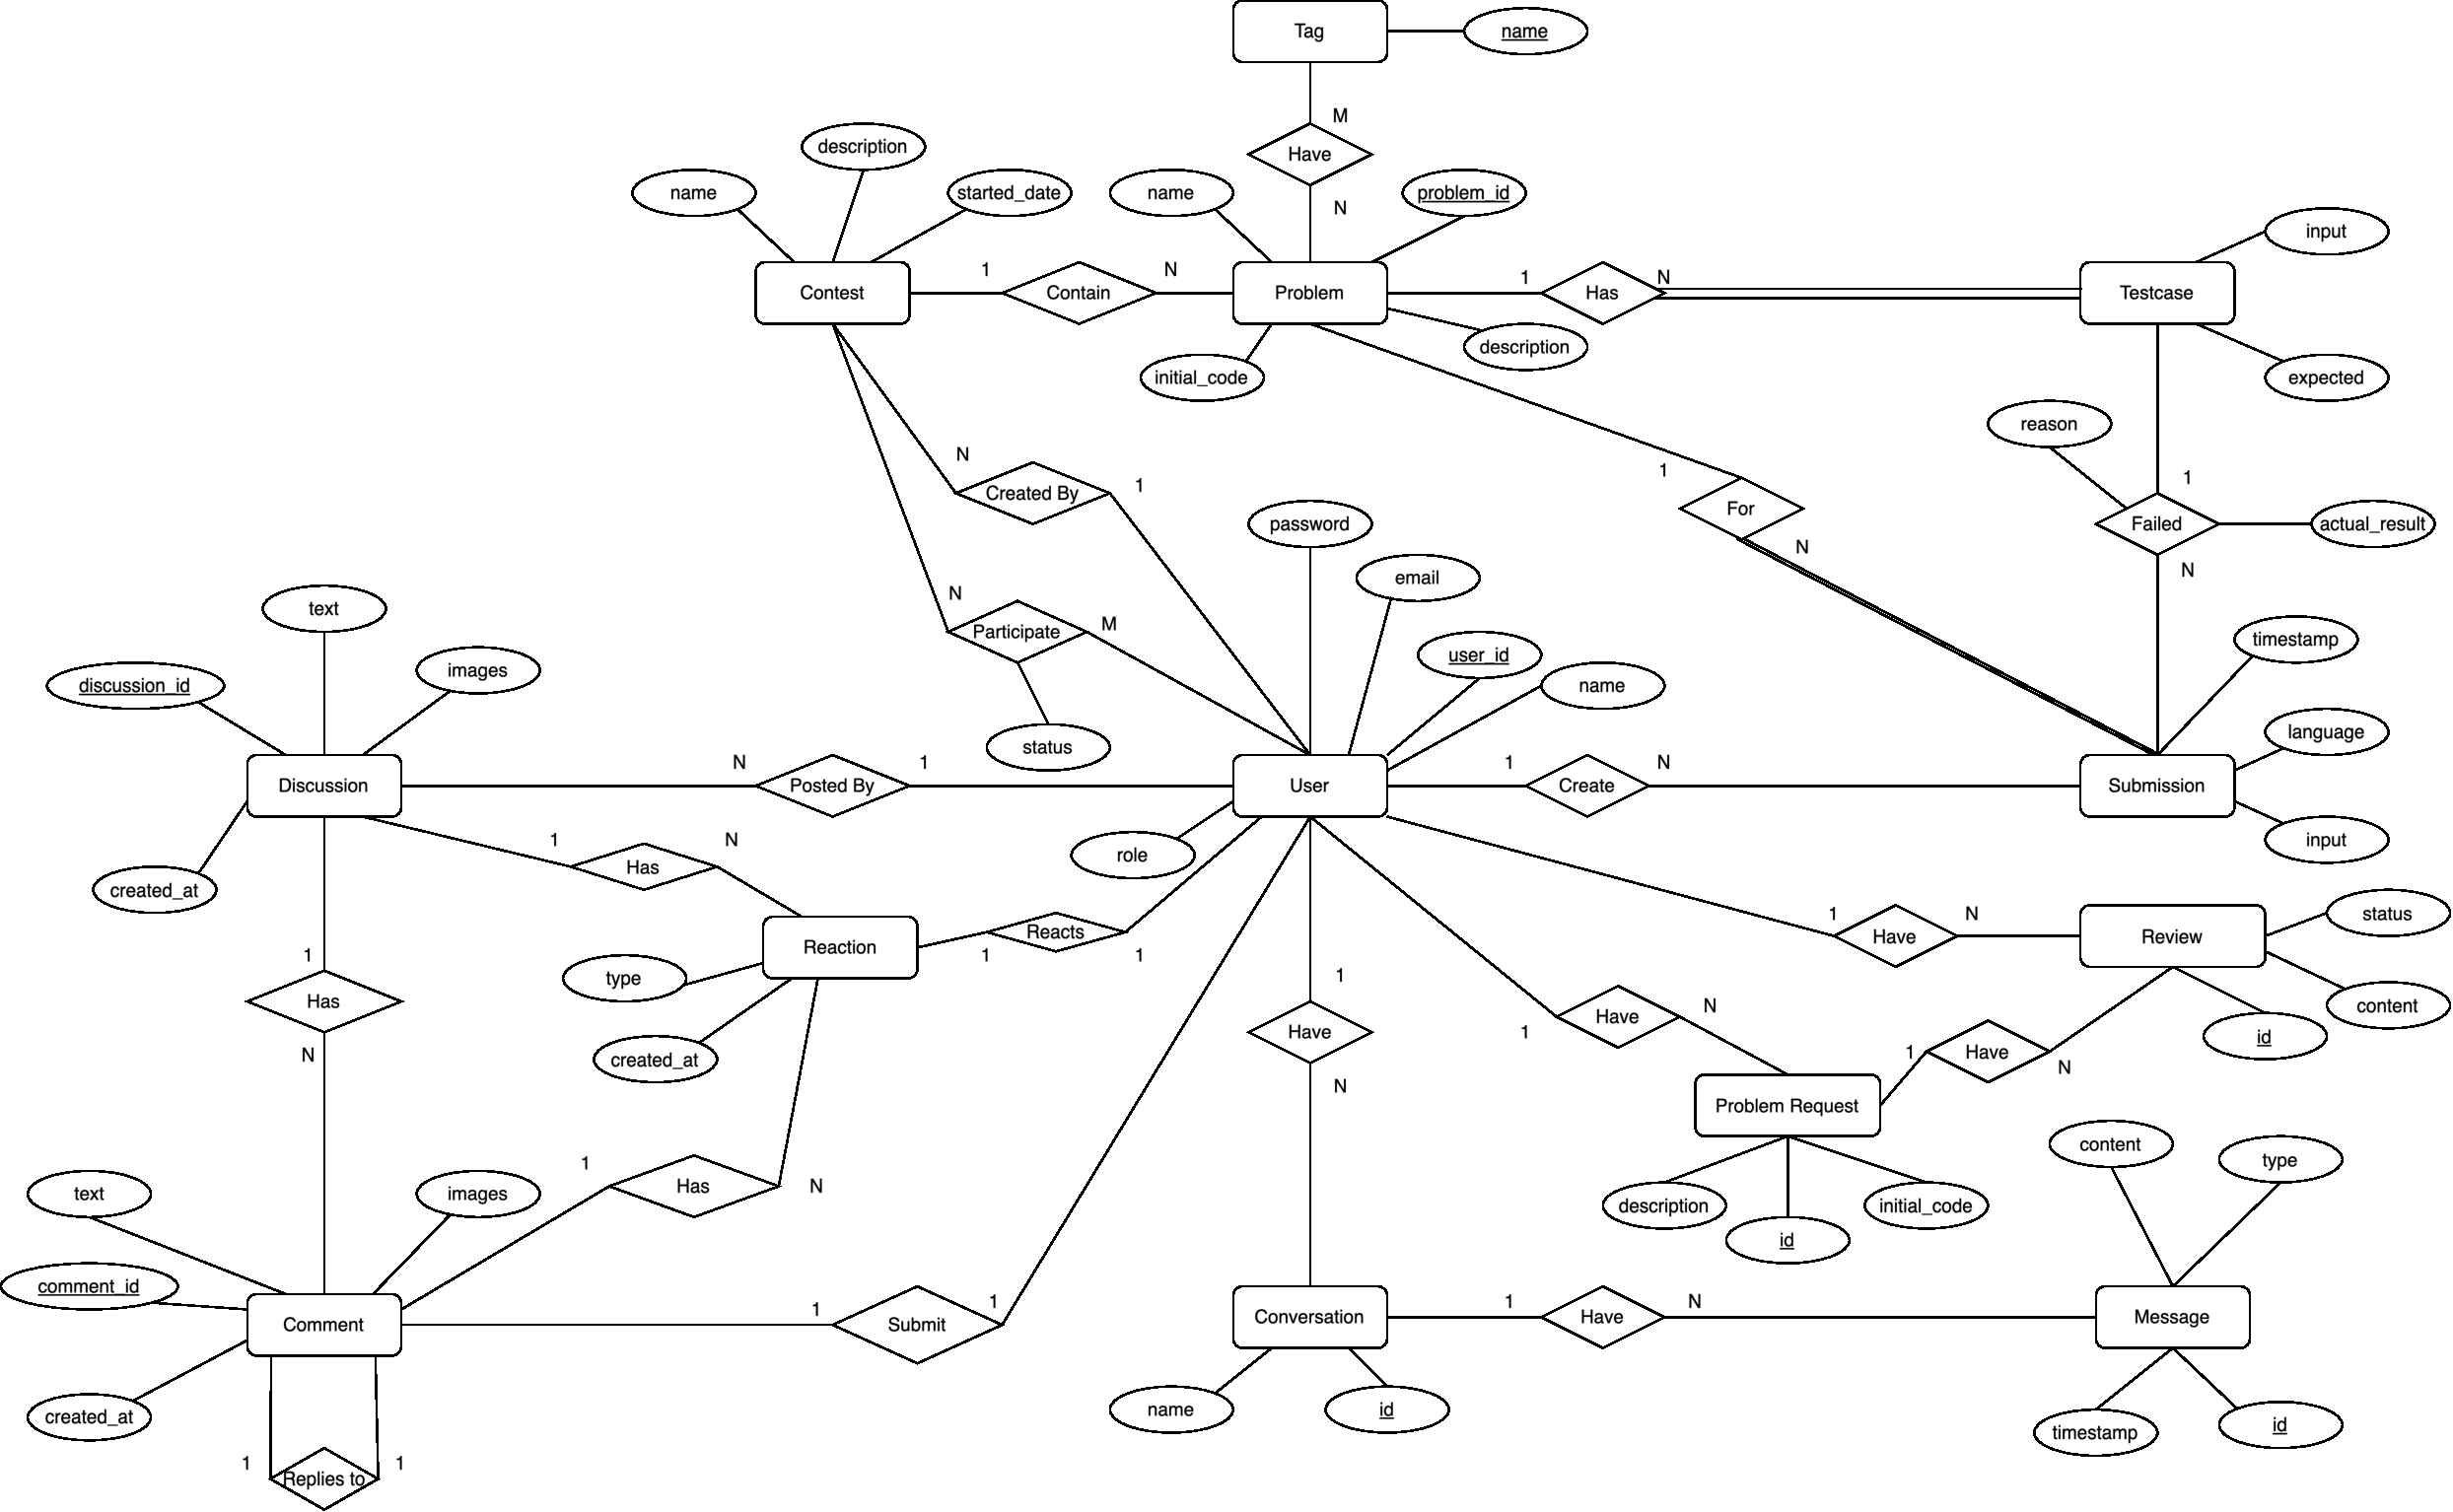
\includegraphics[width=\textheight]{Contents/Chapter 3/Database Design/erd.pdf}}
    \caption{Entity Relationship Diagram}
\end{figure}

\subsection*{User}
\begin{itemize}
    \item \textbf{User}: This abstract entity represents a user of the CodeRank system, storing essential information such as username, email, password hash. Each entity is identified by \textit{user\_id} For simplicity of illustration, we have omitter user roles and permissions in the ERD, all of this is represented by the attribute \textit{role} of the User entity. However, in the actual implementation, user roles and permissions will be managed through Role-Based Access Control (RBAC) to ensure secure and appropriate access to system functionalities.
\end{itemize}

\subsection*{Problems Solving}

\begin{itemize}
    \item \textbf{Problem}: Represents an algorithmic challenge that users can attempt to solve. Each problem includes a unique identifier \textit{problem\_id}, a title, a textual description, and optional starter code (\textit{initial\_code}) to guide users.
A problem may belong to multiple contests and can have multiple tags for classification.
    \item \textbf{Tag}: The \textit{Tag} entity helps organize problems into conceptual groups (for example, Dynamic Programming, String, etc). Each tag has a \textit{name} and may be associated with multiple problems through a many-to-many relationship.
    \item \textbf{Testcase}: Belongs to one problem and includes input data and the corresponding expected output. Testcases are used during code execution to validate user submissions.
    \item \textbf{Submission}: Represents a user's attempt to solve a problem. Each submission is linked to a specific user and problem, and includes the submitted code, programming language, timestamp, and status (e.g., pending, accepted, rejected).
\end{itemize}

\subsubsection*{Problems Management}

\begin{itemize}
    \item \textbf{Problem Request}: Represents a request made by a moderator or superadmin to add a new problem to the platform. Each request includes a title, description, and status (e.g., pending, approved, rejected). It is linked to the moderator or superadmin who made the request.
    \item \textbf{Review}: Represents the review process for a problem request. Each review is associated with a specific problem request and includes feedback, status (e.g., approved, rejected), and the timestamp of the review. It is linked to the moderator or superadmin who conducted the review.
\end{itemize}

\subsection*{Contest}
\begin{itemize}
    \item \textbf{Contest}: Represents a coding competition that users can participate in. Each contest includes a unique identifier \textit{contest\_id}, a title, description, start time, end time, and a list of problems included in the contest. A contest will contain many problems, anc can have many participants.
\end{itemize}

\subsection*{Interview Practice}

\begin{itemize}
    \item \textbf{Conversation}: Represents a coding interview session between a Primary User and chatbot system. Each conversation includes a unique identifier \textit{conversation\_id}, start time, end time. Each conversation is linked to the Primary User who initiated it.
    \item \textbf{Message}: Represents individual messages exchanged during a coding interview conversation. Each message includes a unique identifier \textit{message\_id}, timestamp, content, and type of the message. If the message comes from Primary User, the type will be \textit{user}, otherwise \textit{system}. Each message is linked to the conversation it belongs to.
\end{itemize}

\subsubsection*{Discussion}
\begin{itemize}
    \item \textbf{Discussion}: represents forum-like discussion threads associated with a topic. Users can post questions, explanations, optimization ideas, or clarifications. Each discussion entry may contain text and optional images, and it records creation timestamps.
    \item \textbf{Comment}: Users can comment on discussion threads, forming a threaded conversation system. Each comment includes text, optional images, and a timestamp.
    \item \textbf{Reaction}: Users can react to both discussions and comments using predefined reaction types (e.g., like, love, insightful). Each reaction records the type of reaction and the user who made it.
\end{itemize}

To summarize the relationships among these entities:
\begin{itemize}
    \item A \textbf{User} can \textbf{submit} multiple \textbf{Submission}.
    \item Each \textbf{Submission} is \textbf{linked} to one \textbf{User} and one \textbf{Problem}.
    \item A \textbf{Problem} can \textbf{have} multiple \textbf{Testcases} and can be \textbf{associated} with multiple \textbf{Tags}.
    \item A \textbf{Contest} can \textbf{have} multiple \textbf{Users} as participants.
    \item A \textbf{Contest} can \textbf{include} multiple \textbf{Problem}.
    \item A \textbf{Problem Request} is made by a \textbf{User} with moderator or superadmin role.
    \item A \textbf{Review} is \textbf{conducted} by a \textbf{User} with moderator or superadmin role for a specific \textbf{Problem Request}.
    \item A \textbf{Conversation} is \textbf{initiated} by a \textbf{User} with Primary role.
    \item A \textbf{Conversation} can have multiple \textbf{Messages}.
    \item A \textbf{Discussion} can have multiple \textbf{Comments} and \textbf{Reactions}, and each \textbf{Comment} can also have multiple \textbf{Reactions}.
    \item A \textbf{Tag} can be associated with multiple \textbf{Problems}.
\end{itemize}

